
\documentclass[12pt,a4paper]{article}

\usepackage{fontspec}

\usepackage[BoldFont]{xeCJK}

%\setCJKmainfont{BiauKaiTC}                % 中文字型使用標楷體
\setCJKmainfont{DFKai-SB}
\setmainfont{Times New Roman}          % 如果英文字型是 Times New Roman 則取消這行註解

\XeTeXlinebreaklocale "zh"             % 這兩行一定要加,中文才能自動換行

\XeTeXlinebreakskip = 0pt plus 1pt     % 這兩行一定要加,中文才能自動換行

\usepackage{geometry}

\geometry{
 a4paper,
 left=12.7mm,       %左邊界
 right=12.7mm,      %右邊界
 top=12.7mm,        %上邊界
 bottom=12.7mm,     %下邊界
 }

\usepackage{amssymb}

\usepackage{mathtools}

\usepackage{microtype}

\usepackage{enumitem}

\usepackage{dirtytalk}

\usepackage{subcaption}

\usepackage{fancyhdr}

\usepackage{graphicx}

\usepackage{indentfirst}

\usepackage{hyperref}

\usepackage{zhnumber}

\zhnumsetup{style=Traditional}

\usepackage[backend=biber,style=ieee]{biblatex}

\addbibresource{references.bib}

\AddEnumerateCounter{\zhdig}{\zhdig}{}

\DeclareCaptionLabelSeparator{custom}{、 }

\usepackage[justification=centering,figurename={},tablename={},labelsep=custom]{caption}

\renewcommand{\thetable}{表\zhdig{table}}

\renewcommand{\thefigure}{圖\zhdig{figure}}

\renewcommand{\tableautorefname}{}

\pagestyle{fancy}

\fancyhead{} % 清除所有頁首設定

\fancyfoot{}

\renewcommand{\headrulewidth}{0pt}

\renewcommand{\footrulewidth}{0pt}

\setlength{\headwidth}{\textwidth}

\lfoot{表 C802}

\rfoot{共~~\pageref{LastPage}~~頁~~第{~~\thepage~~}頁}

\begin{document}

\setlength{\parindent}{2em}

\noindent{\bf \large  二、 研究計畫內容:}

\begin{enumerate}[label={(\zhdig*)}, leftmargin=2\parindent, listparindent=\parindent]

\item 摘要

\item 研究動機與研究問題

\begin{enumerate}[label={(\arabic*)}, leftmargin=\parindent, listparindent=\parindent]

\item\textbf{研究問題}

隨著微服務 (Microservices)\cite{1}和雲端原生技術
(Cloud-Native)\cite{2}的普及,現代應用系統高度依
賴高併發應用程式介面 (Application Program Interface, API)
服務,應用於金融交易、電商促銷、影音串流、物聯網等場景,並對 低延遲、
高可用性與動態擴展提出了嚴格要求。例如:

\begin{itemize}[leftmargin=\parindent, listparindent=\parindent]

\item 金融交易 API 需要毫秒級延遲來確保最佳買賣時機,對資源調度
與計算負載有極高要求。交易峰值可能在短短幾秒內增加數十倍,若 API
擴展反應過慢,可能導致交易失敗或市場損失。\cite{3}

\item 大型電商平台促銷活動期間 (如雙 11 促銷活動),大量用戶同時
請求API 進行商品查詢、購物車更新、訂單提交,瞬間請求量可達數百萬每
秒查詢數 (Queries Per Second, QPS)。傳統的 API 擴展方式無法即
時應對流量暴增,可能導致購物車服務崩潰、支付 API 超時,影響用戶體驗
與企業營收。\cite{4}

\item 社群媒體與影音串流 (如 TikTok、YouTube、Instagram)
用戶大量發送請求以獲取動態、影片內容,並伴隨 AI 推薦計算
(如 TikTok For You Feed)。服務需要即時擴展,確保推播
內容的低延遲傳遞,同時兼顧後端機器學習推理任務的負載平衡。\cite{5}

\item 物聯網 (Internet of Things, IoT) 平台
(如智慧城市、工業 4.0) 則是有大量 IoT 設備持續發
送感測數據至雲端 API 進行分析、存儲,且流量具有明
顯的時段性波動 (如白天比晚上流量高)。若 API 無法
適應 IoT 端的流量模式,可能導致數據擷取延遲或設備
無法連接雲端,影響關鍵應用 (如智慧交通信號調度)。\cite{6}

\end{itemize}

然而,目前有許多企業採用 Kubernetes (K8s) 來管理雲端資源,
並透過 Pod 水平/垂直自動擴縮器
(Horizontal/Vertical Pod Autoscaler, H/VPA)
和集群自動擴縮器 (Cluster Autoscaler, CA)
來應對流量變化。然而,這些現有擴展機制在高併發 API
服務場景下仍存在以下關鍵問題\cite{7}:
\begin{itemize}[leftmargin=\parindent, listparindent=\parindent]
    \item\textbf{資源調度延遲:}

H/VPA 依賴中央處理器 (CPU) 或記憶體的用量閾值來監測並觸發 Pod 擴縮,
然而這種方式屬於被動式反應,H/VPA 需要等到 CPU 或記憶體負載超過閾值
後才開始擴展,這意味著系統已經開始過載才會進行調整,並且 H/VPA 整體
擴展過程也會具有一定延遲,從而導致 API 服務短期內請求失敗率上升。

    \item \textbf{
負載預測不準確
}

H/VPA 無法提前預測 API 流量模式,而是單純依賴當下的 CPU 或記憶體使用率,
這在應對突發性高併發流量時顯得效率低下,例如電商促銷開始前的
API 請求量通常會呈指數級增長,但 H/VPA 在負載真正升高前不
會觸發擴展,導致初期請求可能被拒絕。

\item \textbf{無法學習歷史數據:}

H/VPA 不會根據歷史 流量模式來調整策略,無法針對每天固定時段的高峰流量 (如午餐時段、晚間流量高峰)
做出提前擴展的決策。

    \end{itemize}
    \item \textbf{研究動機與目標}

容器調度 (Container Scheduling) 是雲端計算和邊緣計算領域的重要研究
課題,其目標是在動態環境中有效管理資源,確保負載均衡、降低能源消耗
並提升應用效能。現有的研究方法\cite{11}可分為\textbf{數學建模 (Mathematical
Modeling) 、啟發式演算法 (Heuristic Algorithms) 、
元啟發式演算法 (MetaHeuristic Algorithms) 、
機器學習 (Machine Learning) }等不同類別,本節
將基於近期的研究成果進行綜合探討與比較。

\begin{enumerate}[label={(\zhdig*)}, leftmargin=\parindent, listparindent=\parindent]

\item \textbf{啟發式演算法:區域性感知與多目標調度}

啟發式演算法通常透過經驗法則和啟發資訊進行資源分配,較適用於即
時調度需求,但易受局部最優解影響。
\begin{itemize}[leftmargin=\parindent, listparindent=\parindent]
    \item \textbf{
        \cite{12} 區域性感知 (Locality-Aware) 調度}

    Diego 等人提出了一種區域性感知的調度機制,透過
    統計方法將負載均衡 (Load Balancing) 與應用效能 (Application Performance)
    統一為一個優化問題,以降低 I/O 和網路流量瓶頸。該方法適用於資料密
    集型應用,並在 CloudFoundry 平台上驗證了其效能優勢。
    \item \textbf{\cite{13} Multiopt:多目標最佳化調度}

    Multiopt 是一種基於多目標最佳化 (Multi-Objective Optimization) 的調
    度方法,綜合考量 CPU 使用率、記憶體使用率、網路傳輸時間、容器與節
    點的關聯性、容器聚類等五個因素,透過計分函數 (Scoring Function) 選
    擇最佳節點來部署容器,進一步提高系統的每
    秒交易數 (Transactions Per Second, TPS) 並降低平均響應時間。

\end{itemize}
\item \textbf{
    元啟發式演算法:螞蟻、粒子群與混合演算法
}

元啟發式演算法 (Meta-Heuristic Algorithms) 利用啟發資訊進行全域搜
尋,適用於複雜調度問題,但計算開銷較高。
\begin{itemize}[leftmargin=\parindent, listparindent=\parindent]
    \item \textbf{\cite{14} MOO-ACA,GA-MOCA:基於螞蟻演算法 (ACO) 的容器調度}

    MOO-ACA 透過螞蟻演算法 (Ant Colony Algorithm, ACO) 來考量網路
    傳輸開銷、負載均衡與服務可靠性,運用費洛蒙更新機制提升全域最適性,
    使得容器調度更符合雲端環境的變動需求。

    \item \textbf{
        \cite{15} EECS 與 APSO:基於粒子群最佳化的能效調度
    }

    EECS 採用加速粒子群最佳化 (APSO) 演算法,透過權重加總法
    (Weighted-Sum Method) 來同時考量計算時間與能源消耗,並透過\textbf{規則
    式策略 (Rule-Based Strategy) }確保容器分配的合理性,進而降低雲端數
    據中心的總能源消耗。

\end{itemize}
\item \textbf{
    容器虛擬化與軟體定義數據中心 (Software Defined Data Centers, SDDC) 調度策略
}

容器虛擬化技術 (Container-Based Virtualization) 為雲端與邊緣環境提供輕
量級虛擬化能力,並透過動態資源分配提升系統效率。
\begin{itemize}[leftmargin=\parindent, listparindent=\parindent]
    \item \textbf{\cite{16} 基於容器的虛擬化調度模型}

    該研究提出了一種基於容器虛擬化的節能型工作流調度方法,透過雙向
    鏈表訪問機制 (Doubly Linked List-Based Access) 與哈希調度 (Hash-Based
    Scheduling) 來動態管理資源,並減少虛擬機器(Virtual Machine, VM)
    遷移開銷。該方法可在 SDDC 環境下提升能效與系統穩定性。

\end{itemize}
\item \textbf{基於多準則決策分析 (Multi-Criteria Decision Analysis, MCDA)
    的 Kubernetes 容器調度}

MCDA 方法適用於多維度資源調度問題,可透過權
重分析與演算法結合提升決策準確性。
\begin{itemize}[leftmargin=\parindent, listparindent=\parindent]
    \item \textbf{\cite{17} KCSS:基於 MCDA 的 Kubernetes 容器調度策略}

    KCSS 透過理想解相似度順序偏好法
    (Technique for Order Preference by Similarity to an Ideal Solution,
    TOPSIS) 演算法,考量 CPU、記憶體、磁碟使用率、功耗、
    容器數量、影像傳輸時間等六個因素,以排程完成時間 (Makespan) 與能源
    效率為主要目標來優化 Kubernetes 調度決策。

\end{itemize}

\end{enumerate}

綜合前述文獻可知,近年來容器調度已朝多元化方向發展:
從啟發式演算法、元啟發式演算法到容器虛擬化與 SDDC
的協同應用,都在試圖解決動態環境中的資源管理效率問題。
然而,Kubernetes 在面對高併發 API 服務與異構計算
資源時,仍需要更先進的預測與自適應機制。本研究據此提
出以下研究目標 :
\begin{itemize}[leftmargin=\parindent, listparindent=\parindent]
    \item\textbf{整合深度學習與強化學習技術}

大部分現有調度方法強調即時反應與負載均衡,
但對於高併發的動態流量,若無法事先預測負載
波動,將容易陷入資源不足或過量的困境,導致
效能不穩定或資源浪費。因此,本計畫擬設計基於
深度學習 (如 RNN/CNN) 的負載預測模型,並
引入強化學習 (Reinforcement Learning, RL)。

    \item\textbf{服務級別協定 (Service-Level Agreement, SLA) 驅動的自適應 CA}

K8s 既有的 CA 在應對高併發服務時,
往往反應延遲或判斷條件過於簡化。
我們期望透過 SLA (如 API 響
應時間、成功率等指標) 動態驅動
CA,並藉助強化學習與深度學
習推估負載趨勢,使 CA 能實時且
彈性地擴增或縮減叢集資源。

    \item\textbf{提升容器調度效率與 API 響應品質}

在多目標最佳化框架之下,配合元啟發式演算法 (Meta-Heuristic Algorithms)
的調度,讓 Kubernetes 能更準確地選擇最佳節點佈署 Pod。

\end{itemize}

基於這些考量,本研究將著力於「深度學習式負載預測」與「 智能 Kubernetes 調度」的結合,
並融入 SLA 驅動的自適應 CA 機制,以達到高併發 API 服務下的穩定性與資源效率之最優化。

\end{enumerate}
\item 文獻回顧與探討

\begin{enumerate}[label={(\arabic*)}, leftmargin=\parindent, listparindent=\parindent]
\item \textbf{文獻回顧}
\begin{enumerate}[label={(\zhdig*)}, leftmargin=2\parindent, listparindent=\parindent]

\item\textbf{容器化 (Containerization) \cite{9}與虛擬化技術
    (Virtualization) \cite{8}}

早期雲端環境普遍採用虛擬化技術 (Virtualization) ,
透過虛擬機管理程式 (Hypervisor) 將實體伺服器切割成多
個虛擬機 (Virtual Machines, VMs) ,每個 VM 擁有獨
立的作業系統與應用程式堆疊。此種方式雖能顯著提升硬體利用率、
實現熱遷移 (Live Migration) 以及有效的環境隔離,但每個 VM 均
須配備完整作業系統 (OS),資源佔用相對較高。大規模擴展時,
管理多個 VM 也將增加系統複雜度與維運成本。

隨著硬體效能再度提升與微服務化架構的崛起,容器化技術
(Containerization) 成為另一股主流。容器只在應用層
級進行虛擬化,與宿主機 (Host) 共享作業系統核心,
並透過 Linux NameSpaces、cgroups 等機制實現檔案
系統與網路的隔離。此種「進程級 (Process-level) 」虛
擬化具備映像檔體積小、啟動速度快、可移植性與一致性高等
優勢,因此在企業雲、微服務及混合雲領域受到廣泛關注。然而,
容器安全性與隔離度相對於 VM 較低,且在面對大規模佈署、
多雲或邊緣至雲端 (Edge-to-Cloud) 的環境時,容器還需更
完備的編排與資源管理機制 (例如 Kubernetes、Docker Swarm 等) ,
以因應動態負載與需求變化。

近年來,針對容器化雲端資源管理的研究持續增加,
包括容器間隔離、安全強化以及多層次雲端 (Edge/Fog/Cloud)
部署上的協同調度問題。Maenhaut 等人的研究\cite{20} 更進一步點出,
在大規模容器集群下,傳統為 VM 設計的排程及資源配置方案,
若未配合容器的快速啟動與更細顆粒度的資源使用特性,
可能導致效率低落與服務效能不穩定;同時,容器遷移 (Container Migration)
亦需考量應用狀態以及網路延遲等因素。在此背景下,
如何在容器環境中實現高效且安全的彈性擴縮機制,
並確保對 SLA 或 QoS 的遵循,成為容器化雲端研究與應用的重點課題。

\item\textbf{
微服務 (Microservices) \cite{10},雲端原生技術 (Cloud-Native) 與 Kubernetes
}

Kubernetes 是由 Google 在 2014 年以開源方式釋出,
並逐漸成為容器編排領域的事實標準。它能自動化部署、管理、
監控並擴展容器化應用,減少團隊在龐大容器協調工作上的負擔
。Kubernetes 以 Pod 作為運行單元,每個 Pod 內可包含
一個或數個協同運行的容器,並透過如 Service、Deployment、
ReplicaSet 等核心物件實現滾動更新、回滾、故障自動修復與
自動伸縮等功能。在雲端環境中,Kubernetes 採用宣告式 (Declarative) 的方法,
使用者只需描述「期望狀態 (Desired State) 」,系統就會自動將叢集內的容器數量、
部署位置與健康檢查等調整至理想狀態,並與 DevOps、GitOps 及 CI/CD 等工具鏈高度整合。

微服務 (Microservices) 則是一種將大型應用程式拆分為多個
獨立服務模組的軟體架構風格;每個微服務聚焦於單一業務功能並由
不同開發團隊各自維護與部署。相比單體式 (Monolithic) 應用,
微服務在開發過程中能更靈活地選擇技術棧,並可透過容器化打包成
獨立映像;再結合 Kubernetes 等容器編排工具,實現針對特定功能模
組的彈性伸縮,如流量高峰時只擴增「訂單處理」模組,而不影響其他服務。
微服務架構能大幅提高維護效率與迭代速度,並支援跨團隊的敏捷開發,
但也帶來跨服務間資料一致性、版本控制與觀察性 (Observability)
等複雜度,需要額外導入如 API Gateway、Service Mesh、分散式追蹤等基礎設施。

「雲端原生 (Cloud-Native) 」概念則涵蓋了容器、微服務、
動態編排與 API 驅動的雲端基礎設施,並強調在設計之初就要充
分考量雲端環境的特性,如自動伸縮、分散式部署與故障快速恢復等。
傳統單體式應用往往難以適應快速變動的流量需求;相比之下,
雲端原生技術鼓勵開發者將應用拆解為可獨立部署的服務,
並藉助 Kubernetes 完成容器的集中管理和水平伸縮,
配合 CI/CD、自動化運維工具與宣告式基礎設施達到快速交付與版本更新的目標。
此外,多雲 (Multi-cloud) 與混合雲 (Hybrid Cloud) 的環境需求,
也使雲端原生技術在可移植性與跨平台支援方面顯得更加關鍵。

在此背景下,針對 Kubernetes 叢集中的微服務部署與動態資源競爭等問題,
已有多項研究提出優化方案。Ding 等人\cite{21} 便針對「微服務可用度」
、「動態資源競爭」及「共用相依函式庫」等議題,構建了一個整數非線性模型
(Integer Nonlinear Model) ,以達到在有限節點下,
同時滿足微服務的可用性需求並最小化整體成本。
其研究根據每個微服務的應用特性與壅塞狀況動態分配資源,
並藉由改良的基因演算法迅速尋得近似最佳解。實驗結果顯示,
此方法在成本與效能間可取得更佳平衡,
對有大量容器與複雜微服務組合的雲端原生應用來說,具有相當的參考價值。

\end{enumerate}

\item \textbf{文獻探討}

\end{enumerate}
\item 研究方法及步驟
\begin{enumerate}[label={(\arabic*)}, leftmargin=\parindent, listparindent=\parindent]

\item \textbf{
系統架構
}

本研究旨在解決 Kubernetes 在高併發 API 服務中的調度與自適應擴展問題,
其系統架構由三大核心模組組成:負載預測 (Load Prediction)、
調度 (Scheduling) 及自適應擴展 (Adaptive Scaling)。

\begin{enumerate}[label={(\zhdig*)}, leftmargin=\parindent, listparindent=\parindent]
\item \textbf{架構組成}

\begin{itemize}[leftmargin=\parindent, listparindent=\parindent]

    \item \textbf{負載預測模組 (Load Prediction Module):}
    使用遞迴式神經網路 (Recurrent Neural Network, RNN)
    與卷積神經網絡 (Convolutional Neural Network, CNN)
    來預測未來的 API 負載,並提前規劃資源需求
    ,減少 Kubernetes H/VPA 或 CA 擴展延遲,
    以降低 API 響應時間、提高資源利用率,並減少因擴展延遲而導致的服務中斷。

    \item \textbf{元啟發式演算法調度模組
        (Meta-Heuristic Algorithms Scheduling Module):}
    整合自訂 Kubernetes Scheduler\cite{18}來實現更精細化的排程管理。
    透過基因演算法 (Genetic Algorithm, GA) ,
    最佳化 Kubernetes 調度器 (Scheduler),將 Pod 分配至最佳節點,
    提高資源利用率並降低 API 響應延遲。

    \item \textbf{自適應擴展模組 (Adaptive Scaling Module):}
    不同於 Kubernetes 內建的 H/VPA 和 CA 主要依賴 CPU
    或記憶體使用率來決定資源調度\cite{19},
    而是根據 SLA 監測 API 響應時間與請求成功率或依照負載預測模組的規劃,
    自適應調整 CA 擴展策略,以確保高併發 API 服務的穩定性與效能。

    這三大模組彼此協作,確保 API 服務能夠在高併發環境下即時預測負載、
    智能調度資源、動態擴展集群,提升整體效能。

\end{itemize}

    \item \textbf{
系統運作流程}

當 API 請求進入 Kubernetes 叢集時,系統將根據 API 負載變化與資源狀況,
進行動態預測、智能調度與自適應擴展,具體流程如下:

\begin{enumerate}[label={(\arabic*)}, leftmargin=\parindent, listparindent=\parindent]

    \item\textbf{
負載監測與預測}
\begin{itemize}[leftmargin=\parindent, listparindent=\parindent]

    \item 透過 RNN/CNN 模型預測 API 服務的短期與長期流量趨勢,產生負載預測結果。
    \item 依照預測結果決定是否調用 H/VPA 或 CA 擴展模組,
    調整資源擴展策略,確保擴展決策更符合流量模式。

\end{itemize}
    \item\textbf{
智能調度與 Pod 部署}
\begin{itemize}[leftmargin=\parindent, listparindent=\parindent]
    \item 當有新的 API 請求或擴展需求時,
    智能調度模組會透過 GA 演算法,產生最佳的部署 Pod 計畫並回傳給集群使用。
\end{itemize}
\item\textbf{SLA 驅動的自適應擴展}
\begin{itemize}[leftmargin=\parindent, listparindent=\parindent]
    \item 監測 API 響應時間、請求成功率與系統資源使用狀況,判斷是否需要擴展或釋放資源。
    \item 若請求成功率下降,則透過 SLA
    驅動的 CA 擴展策略來動態調整 Kubernetes 集群的節點數量,確保服務穩定性。
\end{itemize}


\end{enumerate}

\end{enumerate}


\item \textbf{
模組詳細說明}
\begin{enumerate}[label={(\zhdig*)}, leftmargin=\parindent, listparindent=\parindent]

    \item \textbf{
調度器 (Scheduler) }

調度器負責根據集群內的即時資源狀況與負載預測結果,
決定 Pod 部署位置。當新的 API 服務請求進入時,
調度器會選擇最適合的節點來部署 Pod,確保資源使用
最佳化與負載均衡。

    \item \textbf{服務壓力預測器 (Service Load Predictor)}

該模組負責監測單一 API 服務的負載變化,
透過機器學習模型預測 1 到 5 分鐘內的流量趨勢,
幫助 H/VPA 提前規劃擴展決策,減少擴展延遲問題。

\item \textbf{集群壓力預測器 (Cluster Load Predictor) }

此模組負責預測整體 Kubernetes 集群的負載趨勢,
透過學習歷史資源使用數據,分析未來 5 到 15 分鐘
的節點資源需求,並提供 CA 參考,以提升 Kubernetes 節點擴展的準確性。

\item \textbf{H/VPA}

當 Pod 內部資源 (如 CPU 或記憶體) 使用率較高時,
H/VPA 會根據即時負載情況自動調整副本數或 Pod 內的資源配額,
避免因為資源不足而導致 Pod 效能下降或請求失敗,減少不必要的擴展。

\item \textbf{集群擴展器 (Cluster Autoscaler)}

該模組根據集群壓力預測結果,動態調整 Kubernetes 集群節點的數量,
確保系統擁有足夠的計算資源應對 API 請求負載,避免因資源不足而導致
API 響應時間增加或請求丟失。

\end{enumerate}
\item \textbf{
系統架構圖}

\begin{figure} [htbp]

\centering

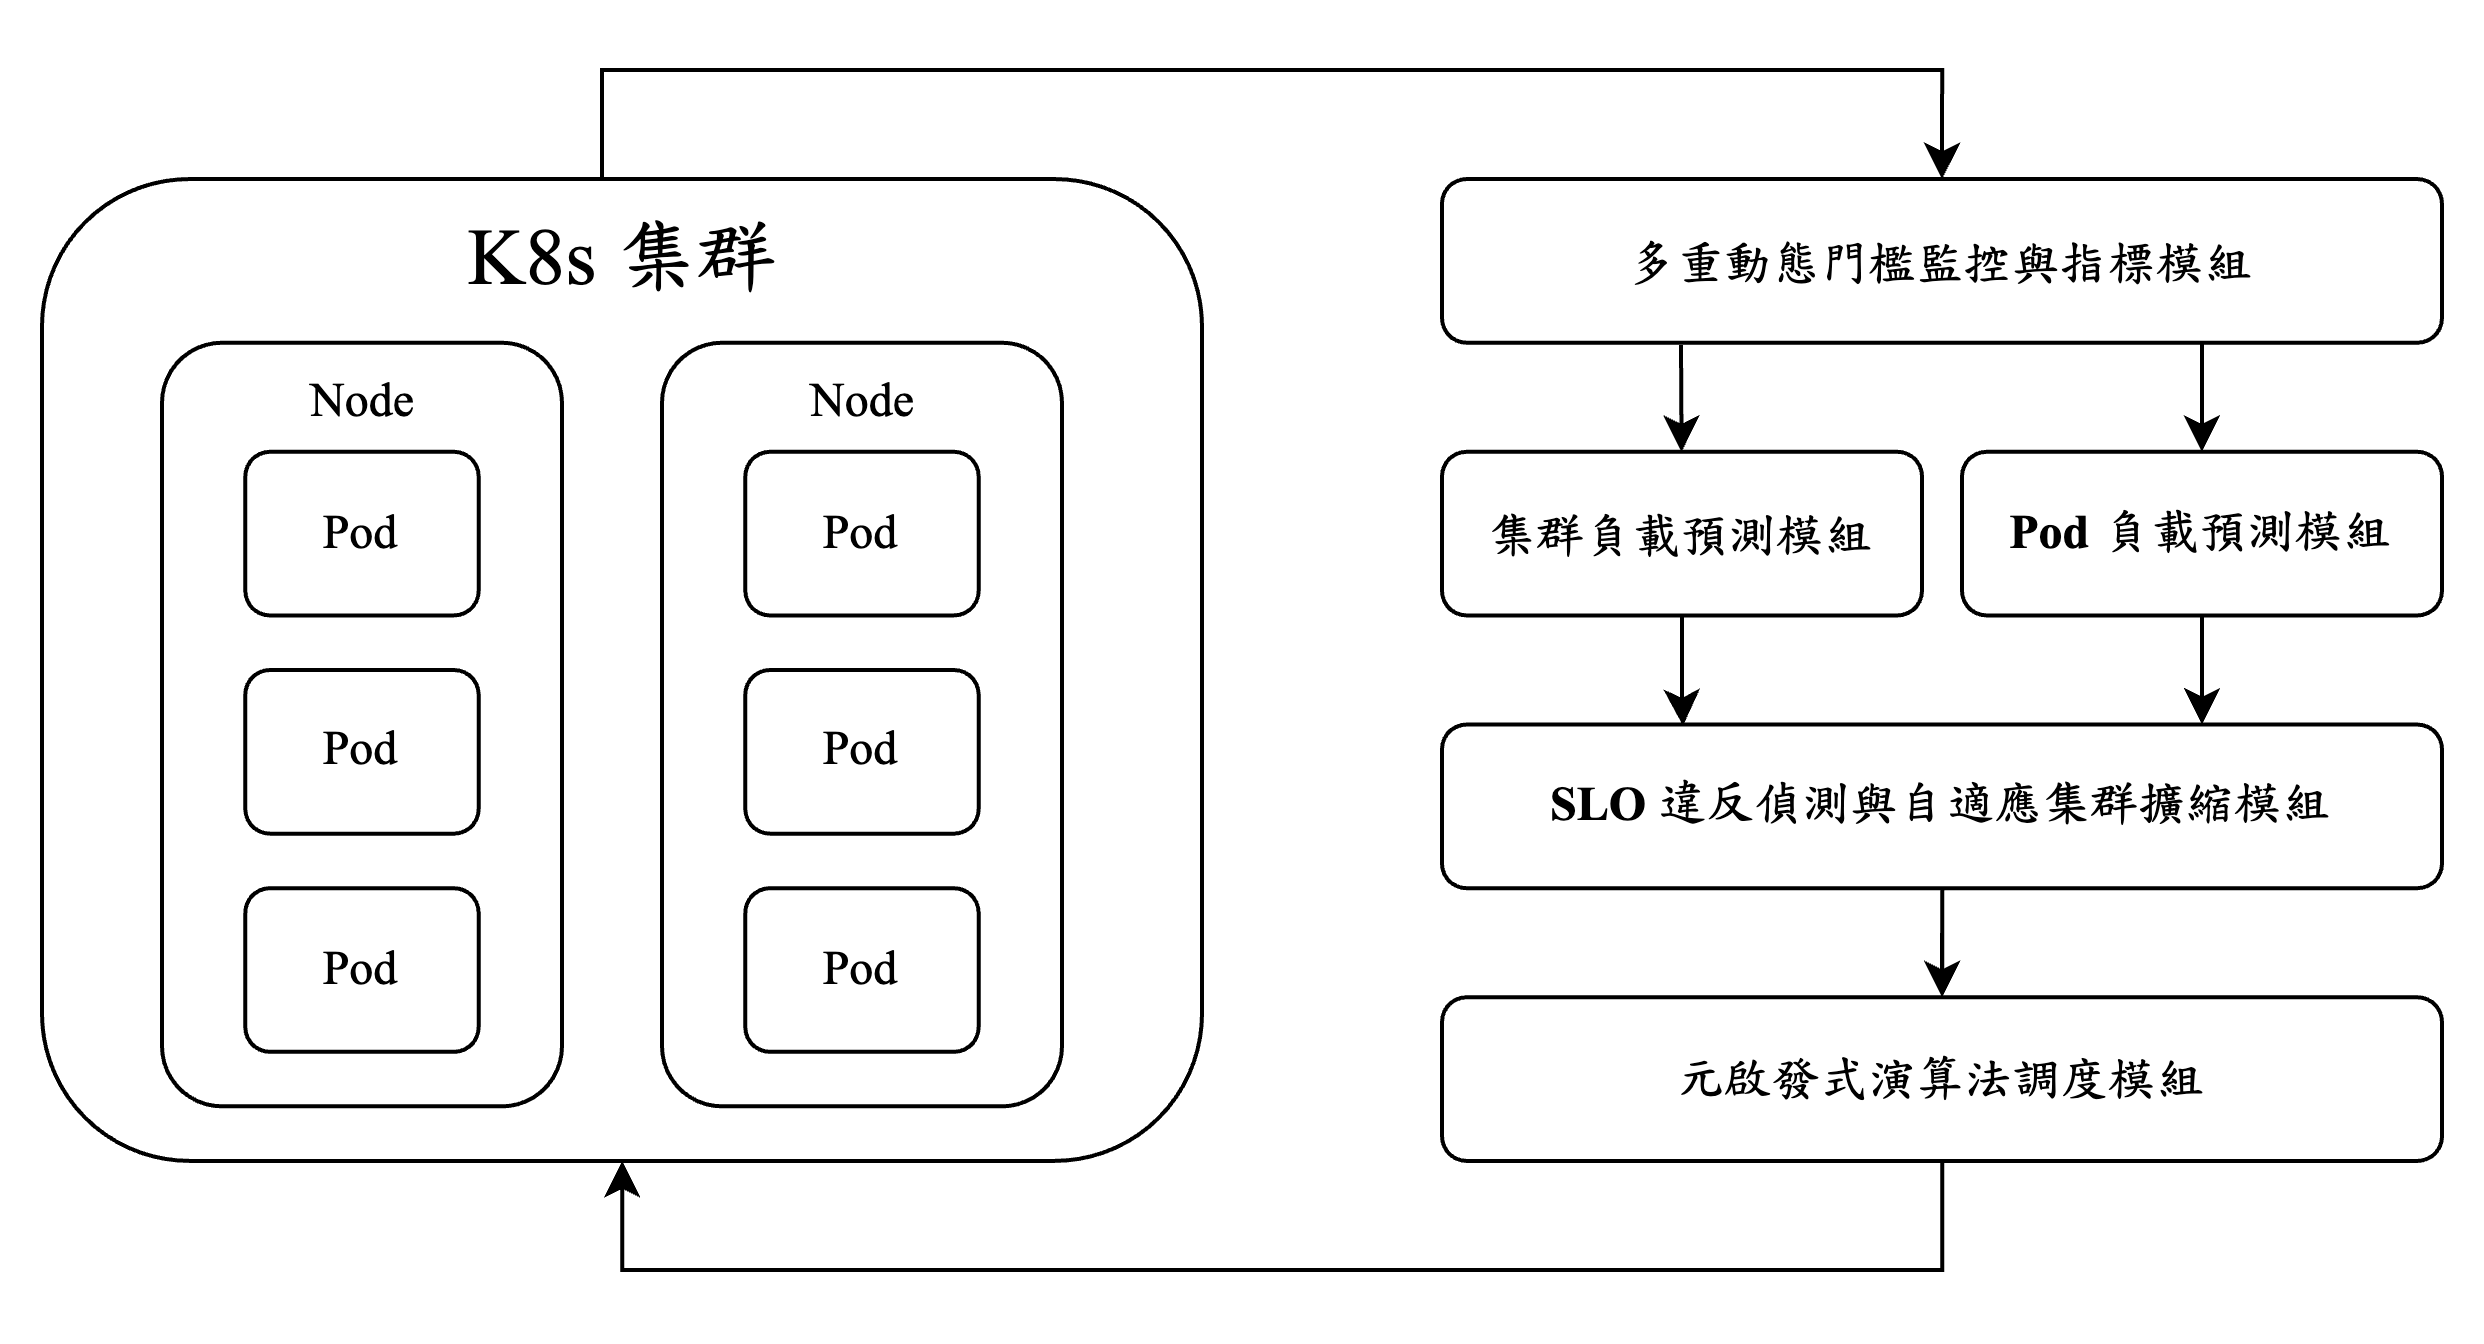
\includegraphics[width=0.9\textwidth]{../fig/model.png}

\caption{架構圖}

\end{figure}\newpage

\end{enumerate}
\item 預期結果

\item 需要指導教授指導內容

\item 參考文獻

\printbibliography[heading=none]

\end{enumerate}


\label{LastPage}


\end{document}

